%\documentclass{standalone}
%\usepackage{tikz, xcolor, pgfplots}

%\begin{document}

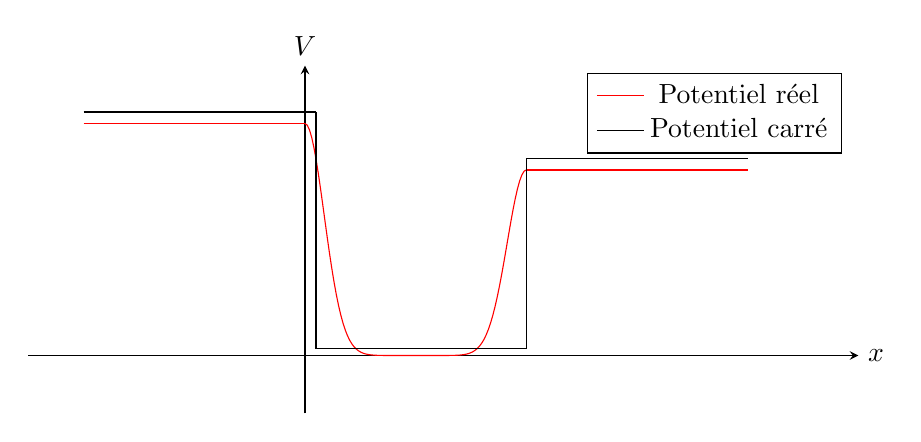
\begin{tikzpicture}
    \begin{axis}[
        xmax = 5,
        xmin = -2.5,
        ymin = -0.5,
        ymax = 2.5,
        axis lines = middle,
        xlabel style = {right},
        ylabel style = {above},
        xlabel = {$x$},
        ylabel = {$V$},
        width=\linewidth,
        height = 6cm,
        ticks = none
        ]
        \addplot[red,domain = 0:2, samples = 100]{2*exp(-x^2/0.06) + 1.6*exp(-(x-2)^2/0.06) };
        \addplot[black, domain = -2:0.1] {2.1} ;
        \addplot[red, domain = -2:0] {2} ;
        \addplot[red, domain = 2:4] {1.6} ;
        \addplot[black, domain = 2:4] {1.7} ;
        \addplot[black, domain = 0.1:2] {0.06} ;
        \addplot[samples = 100] coordinates {(2,0.06)(2,1.7)} ;
        \addplot[samples = 100] coordinates {(0.1,0.06)(0.1,2.1)} ;
        \legend{Potentiel réel, Potentiel carré} ;
        
        
    \end{axis}
\end{tikzpicture}
%\end{document}